\documentclass[english,a4paper,10pt,twoside]{book}

% Language

\usepackage[utf8]{inputenc}
\usepackage[T1]{fontenc}
\usepackage[english]{babel}

% Math

\usepackage{mathtools, amssymb, exscale, mathrsfs}
\usepackage{nicefrac}
\usepackage{units}

\let\originalleft\left
\let\originalright\right
\renewcommand{\left}{\mathopen{}\mathclose\bgroup\originalleft}
\renewcommand{\right}{\aftergroup\egroup\originalright}

% New definition of square root:
% it renames \sqrt as \oldsqrt
\let\oldsqrt\sqrt
% it defines the new \sqrt in terms of the old one
\def\sqrt{\mathpalette\DHLhksqrt}
\def\DHLhksqrt#1#2{%
	\setbox0=\hbox{$#1\oldsqrt{#2\,}$}\dimen0=\ht0
	\advance\dimen0-0.2\ht0
	\setbox2=\hbox{\vrule height\ht0 depth -\dimen0}%
	{\box0\lower0.4pt\box2}}

% Layout

\usepackage[onehalfspacing]{setspace}
\usepackage{titling}
\usepackage{lmodern}
\usepackage[]{hyperref} % hidelinks to hide links :D
\usepackage[a4paper]{geometry}
\usepackage{graphicx}
\usepackage{xcolor}
\usepackage[sort&compress]{cleveref}
\usepackage{paralist}
\usepackage{listings}
\usepackage{rotating}

% Tikz

\usepackage{tikz}
\usetikzlibrary{backgrounds}
\usetikzlibrary{calc}

\setlength{\parindent}{0cm}
\pagestyle{plain}
\author{Fabian Glatzel}
\title{Calculation of tight binding parameters with density functional theory to describe transport phenomena}
\date{\today}
\hypersetup{
  pdftitle=\thetitle von \theauthor,
  pdfauthor=\theauthor,
  colorlinks=false}

\begin{document}
\begin{titlepage}
 \centering 
 \Huge\thetitle\\ 
 
 \vspace*{1cm}
 
 \Large Bachelor Thesis\\
 \vspace*{5cm}
 
 
\includegraphics[width=10cm]{Images/logo_freiburg}
 
 \vspace*{5cm}
 \theauthor
 \normalsize 
\end{titlepage}
\thispagestyle{empty}

\tableofcontents
\pagenumbering{Roman}

\chapter{Introduction}
\pagenumbering{arabic}
\section{Motivation}
The big relevance of transport phenomena in organic semiconductors can be understood by looking at the variety of its applications including photovoltaic, OLED's and many more. 

\section{Theoretical Background}

\subsection{Density Functional Theory}
The informations of this section are mainly based on \cite{KOSKINEN2009237,1402-4896-2004-T109-001}.\\
\emph{Density functional theory} (DFT) is an efficient computational, \emph{ab initio}, self consistency method to calculate quantum mechanical ground states and its properties. Since an analytical solution to Schrödinger's equation can only be found in the simplest cases, but quantum mechanical effects gain more and more relevance in many fields including nanoelectronics and modern materials sciences, DFT comes in very handy.\\
A simple look at the many body Schrödinger equation with the electron positions $\vec{r}_i$ and the core positions $\vec{R}_j$
\begin{align}
	\mathcal{H} \Psi\left(\vec{r}_1,\vec{r}_2,\dots,\vec{r}_N,\vec{R}_1,\dots,\vec{R}_M\right) &= E \Psi\left(\vec{r}_1,\vec{r}_2,\dots,\vec{r}_N,\vec{R}_1,\dots,\vec{R}_M\right)
\end{align}
shows one of the big problems, since this expression is $3(N+M)$-dimensional.
At first the \textsc{Born-Oppenheimer} approximation is applied, stating that the timescale of changing dynamics for the light electrons is much shorter then for the heavy cores and therefore the cores can be assumed to be fixed at their positions to calculate the electrons ground state. This only reduces the problem to $3N$ dimensions.\\
Here comes in the \textsc{Hohenberg-Kohn} theorem, which states that the complete electron ground state density
\begin{align}
n_0\left(\vec{r}\right) = N\int\dd\vec{r}_2\ \dots\int\dd\vec{r}_N\ \left|\Psi_0\left(\vec{r}, \vec{r}_2, \dots,\vec{r}_N,\right)\right|^2
\end{align}
determines the external potential (for example the \textsc{Coulomb} potentials of the cores) and thus the electron ground state wave function $\Psi_0$. Mathematically this means that the wave function is a unique functional of the electron density with $\Psi_0\left(\vec{r}\right) = \Psi\left[n_0\left(\vec{r}\right)\right]$ and consequently every observable can be obtained as a functional of the electron density (therefore the name 'Density Functional Theory').\\
Of course this includes the energy observable $E[n\left(\vec{r}\right)]$, which becomes minimal for the correct ground state $n_0\left(\vec{r}\right)$. Thus the dimension of the problem is reduced to $3$, but causes a new problem, since even if it's known that this functional exists, it contains terms of unknown form due to electron-electron interaction.\\
To resolve this problem, a system with the same electron density out of non directly interacting electrons is assumed. In other words, a system of wave functions $\varPhi_i$ (the so called \textsc{Kohn-Sham} orbitals) is assumed with:
\begin{align}
n\left(\vec{r}\right) &= \sum_i \left|\varPhi_i\right|^2
\end{align}
This wave functions are eigenfunctions to single particle Hamiltonians depending on the electron density $n(\vec{r})$. Again this Hamiltonians contain an unknown term due to many particle interactions, called the \emph{exchange correlation} (XC) term, but this one can be approximated quite good for most purposes. Thus separated equations depending on the electron density $n\left(\vec{r}\right)$ for the single particle wave functions were obtained, which contribute themselves to the electron density $n\left(\vec{r}\right)$. These equations can be solved by iteration and checking for self consistency.\\
Through numerical optimization (minimization) of the ground state energy in respect to the core positions it is also possible to find the relaxed core positions.\\
To get the band structures the single particle eigenvalues with a constrained periodic behavior according to \textsc{Blochs} theorem were calculated (see \cref{section_bloch}).\\
Finally, calculations with manually shifted charges will be performed using \emph{constrained DFT} (cDFT). This is done by defining $i$ regions containing one or multiple cores with positions $\vec{R}_j$ and an absolute charge $N_i$ for each region. The charge of any region is calculated by integrating the electron density $n\left(\vec{r}\right)$ multiplied whit a sum of \textsc{Gaussian} curves centered at the atom positions $R_j$ for all cores in the $i$-th region (see \cref{image_region_gaussians}):
\begin{align}
w_i\left(\vec{r}\right) &= \sum_j w\left(\vec{r} - \vec{R}_j\right) \text{\quad}
\end{align}
This can be written as minimization problem of the cDFT energy $F[n\left(\vec{r}\right), V_i]$:
\begin{align}
F\left[n\left(\vec{r}\right), U_i\right] &= E_0\left[n\left(\vec{r}\right)\right] + \sum_i U_i\left(\int\dd\vec{r}\ w_i\left(\vec{r}\right)\ n\left(\vec{r}\right) - N_i\right)
\end{align}
with the energy functional of the undisturbed system $E_0\left[n\left(\vec{r}\right)\right]$ and the constraints:
\begin{align}
0 &= \int\dd\vec{r}\ w_i\left(\vec{r}\right)\ n\left(\vec{r}\right) - N_i
\end{align}
for all $i$ regions.
The same \textsc{Gaussian} curves are used as external potentials with additional prefactors $U_i$ scaling the strength of the potentials to change the density and thus get the correct charges in each region\footnote{In this way the $U_i$ can be understood as \textsc{Lagrange} multipliers for the minimization problem of the energy with the constraints of a fixed charge in each region.}. The standard deviation $\sigma$ of the \textsc{Gaussian} curves is left as free parameter. The choice of an appropriate value for $\sigma$ will be discussed later (see \cref{section_constraint_density_functonal_theory}).\\
For the calculations in this thesis the Python DFT package \emph{GPAW} (see \cite{GPAW1, GPAW2}) in combination with the atomic simulation environment \emph{ASE} (see \cite{ASE}) is used. Especially the \emph{PBE} (named after \textsc{Perdew Burke} and \mbox{\textsc{Ernzerhof}}) XC functional is used, which is a functional of the electron density $n\left(\vec{r}\right)$  and its gradient. Further the calculations were performed on a real space grid in the manner of a finite difference method.
\begin{figure}
	\centering
	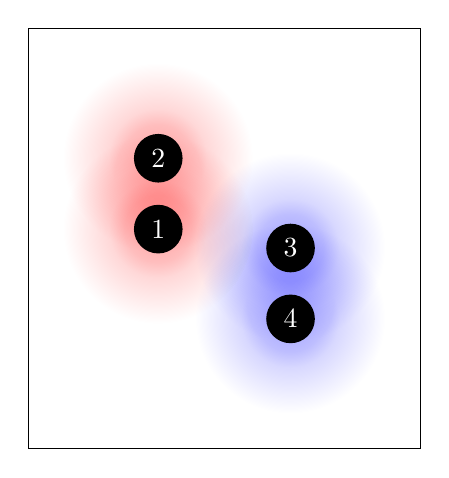
\begin{tikzpicture}[show background rectangle, scale = 0.6]
	\foreach \i/\j/\color in {0/0.2/red, 0/1.7/red, 2.8/-0.2/blue, 2.8/-1.7/blue}{
		\foreach \r in {0, 0.01, ..., 1}{
		 	\fill[opacity = \r * 0.01, fill = \color] (\i, \j) circle ({2.5 * (1 - \r)});}}
	\foreach \i/\j/\num in {0/0.2/1, 0/1.7/2, 2.8/-0.2/3, 2.8/-1.7/4}{
	\node[fill = black, shape = circle, text = white] at (\i, \j)	 {\num};}
	\end{tikzpicture}
	\caption{Scheme: Sum of \textsc{Gaussian} curves for two regions (\textcolor{red}{red} and \textcolor{blue}{blue}), each with two cores (\{1, 2\} and \{3, 4\}), used as weights for the integration/summation over the electron density to calculate the charge in each region.}
	\label{image_region_gaussians}
\end{figure}


\subsection{Lattice}
In the following four sections the informations are basically from \cite{ashcroft} if not otherwise mentioned.\\
A solid has typically a periodicity in the placing of its atoms. This property is called \emph{crystal structure}, which can be locally restricted due to occurring crystal defects. Exceptions are the amorphous solids, which behave like very viscous fluids and will not be discussed here (see \cite{gerthsen}).\\
In the simplest case the atom positions can be described by a \emph{\textsc{Bravais} lattice}. This is a perfectly periodic lattice, where the arrangement and orientation of all atoms look exactly the same from all atom positions (see \cref{image_2D_Bravais}). Therefore the positions $\vec{R}$ of the atoms can be described by:
\begin{align}
	\vec{R} &= \sum_{i = 0}^{N_D} n_i \vec{a}_i
\end{align}
with linearly independent primitive vectors $\vec{a}_i$, $n_i \in \mathbb{Z}$ and the dimension $N_D$.\\ Often the atom positions do not fulfil this condition but unit cells containing multiple atoms do. Thus additional information about the position of the atoms within the unit cell is needed to characterise the structure. This is called a lattice with a \emph{basis}. An one dimensional example can be seen in \cref{image_Bravais_Basis} showing a chain with alternating distances. Here a minimal unit cell (called \emph{primitive cell} or \emph{primitive unit cell}) contains two points and therefore a basis with two basis vectors $\vec{b}_1$ and $\vec{b}_2$. The primitive cell itself fulfils the condition of a Bravais lattice with primitive vector $\vec{a}_1$. If there were no alternation in the chain and all points were equally spaced, the points would form a Bravais lattice themselves with a primitive vector of half the length of $\vec{a}_1$. This will be of importance later in \cref{chapter_Peierls_SSH}.\\
It should be mentioned that a primitive call can always be constructed by simply taking all space closer to a certain lattice point then to all others. This kind of primitive cells are called \emph{\textsc{Wigner-Seitz} primitive cells}.\\
The set of wave vectors $\vec{K}$, that have the periodicity of a given \textsc{Bravais} lattice $\vec{R}$, explicitly:
\begin{align}
\exp\left(\ii\vec{K}\cdot\vec{r}\right) &= \exp\left[\ii\vec{K}\cdot\left(\vec{r} + \vec{R}\right)\right] &\Leftrightarrow& &\vec{K}\cdot\vec{R} &= \mathbb{Z}\cdot 2\pi	
\end{align}
do also form a \textsc{Bravais} lattice in the reciprocal space, the so called \emph{reciprocal lattice}. The \textsc{Wigner-Seitz} primitive cell of the reciprocal lattice, namely the \emph{First \textsc{Brillouine} Zone}, will be relevant for the next section.

\begin{figure}
	\centering
	\begin{subfigure}{0.33\textwidth}
	\begin{tikzpicture}[show background rectangle]
		\foreach \i in {0, 1,...,4}{
			\foreach \j in {0, 1,...,2}{
				\draw[fill = black] ({\i + 0.2 * \j, \j}) circle (0.05);}}
		\draw[-{Latex[scale = 1.2]}] (1.2 ,1) -- (2.2,1) node[midway, below] {$\vec{a}_1$};
		\draw[-{Latex[scale = 1.2]}] (1.2 ,1) -- (1.4,2) node[midway, left] {$\vec{a}_2$};
	\end{tikzpicture}
	\caption{Two dimensional \textsc{Bravais} lattice with primitive vectors $\vec{a}_1$ and $\vec{a}_2$}
	\label{image_2D_Bravais}
	\end{subfigure}\hspace*{2cm}
	\begin{subfigure}{0.33\textwidth}
	\vspace*{0.1cm}
	\begin{tikzpicture}[show background rectangle]
	\foreach \i in {0, 1, 2}{
		\foreach \j in {-1, 1}{
			\draw[fill = black] ({2 * \i + 0.4 * \j, 0}) circle (0.05);}}
	\foreach \i in {0.5, 1.5}{
		\draw[dotted] (2 * \i, 1) -- +(0, -1.05);}
	\draw[-{Latex[scale = 1.2]}] (1 ,1) -- (3, 1) node[midway, above] {$\vec{a}_1$};
	\draw[-{Latex[scale = 1.2]}] (1 ,0) -- (0.4, 0) node[midway, above] {$\vec{b}_1$};
	\draw[-{Latex[scale = 1.2]}] (1 ,0) -- (1.6, 0) node[midway, above] {$\vec{b}_2$};
	\draw (1, -.1) -- (1, .1);
	\end{tikzpicture}
	\caption{One dimensional \textsc{Bravais} lattice with a basis \{$\vec{b}_1, \vec{b}_2$\}}
	\label{image_Bravais_Basis}
\end{subfigure}
\caption{Schemes of \emph{\textsc{Bravais} lattices}}
\end{figure}

\subsection{Bloch Theorem}
\label{section_bloch}
According to \textsc{Bloch's} theorem a wave function $\Psi(\vec{r})$ of a periodic potential, $V\big(\vec{r} + \vec{R}\big)= V\big(\vec{r}\big)$ for all $\vec{R}$ of a \textsc{Bravais} lattice, can be written in the form:

\begin{align}
	\Psi(\vec{r}) &= \exp\left(\ii\vec{k}\cdot\vec{r}\right) \cdot u\left(\vec{r}\right)
\end{align}
where $\vec{k}$ is an arbitrary wave vector and $u\left(\vec{r}\right)$ denotes a $\vec{R}$-periodic function.\\
Under the assumption, that the boundary condition at the surface should not change the physical properties of the bulk, one assumes the periodic \emph{\textsc{Born-von Karman} boundary condition}\footnote{Alternatively one can choose the boundary condition  for a vanishing wave function on the surface $\Psi\left(\vec{S}\right) = 0$. But the periodic boundary condition has the advantage, that it corresponds with propagating waves, which suite transport phenomena very well, whereas a vanishing boundary condition corresponds with standing waves.}:
\begin{align}
	\Psi\left(\vec{r} + N_i \vec{a}_i\right) &= \Psi\left(\vec{r}\right)
\end{align}
where $N_i$ denotes the number of unit cells in the direction $\vec{a}_i$ of the bulk. Hereby one obtains an additional condition for the wave vectors $\vec{k}$, namely:
\begin{align}
	\vec{k} &= \sum_{i = 1}^{N_D} \frac{m_i}{N_i} \vec{b}_i & m_i \in \mathbb{Z} 
\end{align}
It can be shown that if two states only vary in the way that $\vec{k}_1 - \vec{k}_2 \in \vec{K}$, they correspond to the same physical state. The conclusion is that one has to take only the states within the first \textsc{Brillouine} zone into account for a complete description. One considers that the number of states in the first \textsc{Brillouine} zone equals the number of sites $N = \prod_{i = 1}^{N_D}N_i$ of the bulk. For the one dimensional case this means, that the number of states within the first \textsc{Brillouine} zone is the number of primitive cells in the chain.\\
Since there are multiple solutions to \textsc{Schrödinger's} equation for a given $\vec{k}$, they will be labeled by some additional index $n$. In solid state physics the number of atoms contained in a system is usually very big, what corresponds to a high density of states in the reciprocal space. As limit a continuum of states can be assumed in the reciprocal space, which leads to a continuum of eigenenergies in some interval (\emph{band}), since the \textsc{Schrödinger} equation changes continuous with $\vec{k}$. Therefore $n$ is referred to as \emph{band index}. Two bands of special interest are the \emph{HOMO}-band (referring to the 'highest occupied molecular orbital') and the \emph{LUMO}-band (referring to the 'lowest unoccupied molecular orbital').

\subsection{Tight-Binding Method}
In the previous section the eigenstates have been calculated by using the translational symmetries of a \textsc{Bravais} lattice, which results in completely delocalized states. A complete different approach is the following:\\
If the distance between adjacent atoms is much bigger than the typical width of the electron wave functions for isolated atoms, the wave functions shouldn't differ much from that states. By decreasing the distance between the atoms, the electrons will start to feel the presence of the other atoms and will therefore change their states. The tight-binding method handles the case in which the interaction doesn't completely change the wave functions, but the effects are to big to neglect. Since the tight-binding method is a single particle model, it seems quite suitable for the \textsc{Kohn-Sham} orbitals and therefore for the description of the band structures.\\
Mathematically, one starts with the basic single atom Hamiltonian $\mathcal{H}_{\text{at}}$ and it's single particle eigenfunctions $\varphi_n$ satisfying the Schrödinger equation of an isolated atom:
\begin{align}
	\mathcal{H}_{\text{at}} \varphi_n &= E_n \varphi_n
\end{align}
In the next step a second term is added to the Hamiltonian, that applies the corrections needed to describe the lattice correctly. In an one dimensional chain with atom positions $\vec{R}_i$ the modified Hamiltonian contains a term describing the interaction $U$ of adjacent valence electrons with the matrix elements $M_{i, i\pm1}$:
\begin{align}
	M_{i, i\pm1} &= \int\dd\vec{r}\ \varphi_n^*\left(\vec{r} - \vec{R}_i\right)\ U\ \varphi_n\left(\vec{r}-\vec{R}_{i\pm1}\right) 
\end{align}
In can be shown that this term is negative if the wave functions have the same sign where they meet and therefore form a binding state (see \cite{rohrer}). Hence the positive so called \emph{hopping parameter} $t_{i, i\pm 1} = - M_{i, i\pm 1}$ is introduced. In terms of second quantization this interaction Hamiltonian can be written as\footnote{neglecting spin degree of freedom}:
\begin{align}
	- \sum_i t_{i, i+1} \left(c_i^\dagger\  c_{i+1} + c_{i+1}^\dagger\  c_i\right)
\end{align}
with the creation and annihilation operators $c^\dagger_i, c_i$ for an electron located at the $i$-th atom. Thus the term $c_i^\dagger c_{i\pm1}$ can be interpreted as shifting an electron from the ($i\pm1$)-th atom to the $i$-th atom which explains the name hopping parameter for $t$.\\
The combination of the single atom Hamiltonian $\mathcal{H}_\text{at}$ and the next-neighbor-hopping term in the basis of the single atom wave functions $\varphi_n$ for the $i$ atoms can than be written as:
\begin{align}
	\mathcal{H} &= \sum_i E_n n_i - \sum_i t_{i, i+1} \left(c_i^\dagger\  c_{i+1} + c_{i+1}^\dagger\  c_i\right)
\end{align}
with the number operator $n_i = c^\dagger_i c_i$, that simply returns the number of electrons in the state $\varphi_n$ of the $i$-th atom. In matrix notation this Hamiltonian would look like:
\begin{align}
	\mathcal{H} &= \begin{pmatrix*}
	\ddots&&&\\
	&E_n&-t_{i-1, i}&0\\
	&-t_{i, i-1}&E_n&-t_{i, i+1}\\
	&0&-t_{i+1, i}&E_n&\\
	&&&&\ddots
	\end{pmatrix*}
\end{align}
In the simple case of equally spaced atoms with distance $a$ all hopping parameters become the same $t_{i, i\pm1} = t\quad\forall  i$. 

\subsection{Peierls Distortion and SSH-Hamiltonian}
\label{chapter_Peierls_SSH}
\textsc{Peierls} instability theorem states, that an one-dimensional chain of atoms with a single unpaired electron will always distort from a perfect periodic placing of its atoms (see \cite{chandrasekhar,nalwa}). Or in other words, breaking the symmetry under the previous told conditions will lower the ground state energy.\\
Thus a displacement $u_n$ of the atoms is expected yielding the new atom positions:
\begin{align}
	R_n &\mapsto (-1)^{n}u_n + R_n
\end{align}
As a consequence also the hopping-parameter will be effected in the way $t_{n, n+1} = t_0 + \delta_n$ and for small displacements $u_n$ the linear approximation $\delta_n = \alpha (u_{n+1} - u_n)$ with the \emph{phonon coupling constant} $\alpha = \nicefrac{\partial t}{\partial u}$ will hold.\\
An important example which includes this hopping-term is the Hamiltonian used to describe the electron-hopping in \emph{trans}-polyacetylene (see \cref{image_trans_polyacetylene}). Here $u_n$ describes the displacement of a CH group.\\
\begin{figure}
	\begin{minipage}{0.49\textwidth}
	\centering
	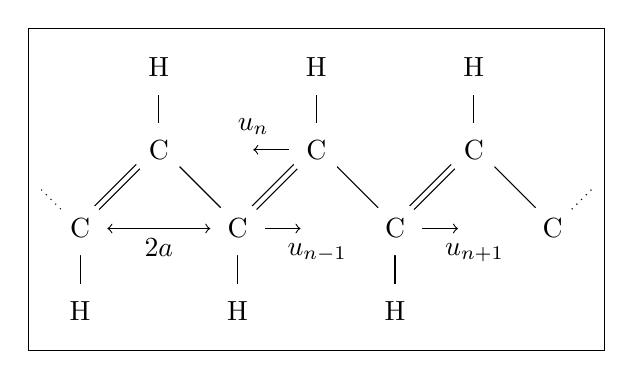
\begin{tikzpicture}[show background rectangle, scale = 1]
		\foreach \i in {0,2,4}{
			\draw (\i, 0) -- +(1,1);
			\draw (\i, 0.1) -- +(1,1);
			\draw (\i + 1, 1.05) -- +(1, -1);
			\draw (\i, 0) -- +(0,-.7) node[circle, fill = white, below] {H};
			\draw (\i + 1, 1) -- +(0,.7) node[circle, fill = white, above] {H};
			\node[circle, fill = white] (d\i) at (\i, 0) {C};
			\node[circle, fill = white] (u\i) at (\i + 1, 1) {C};
			}
		\draw [<->] (d0) -- (d2) node [midway, below] {$2a$};
		\draw [->] (d2) -- +(.8, 0) node [below, xshift = 6, yshift = -2] {$u_{n-1}$};
		\draw [->] (d4) -- +(.8, 0) node [below, xshift = 6, yshift = -2] {$u_{n+1}$};
		\draw [->] (u2) -- +(-.8, 0) node [above, yshift = 2] {$u_{n}$};
		\node[circle, fill = white] (end) at (6,0) {C};
		\draw [dotted] (end) -- +(.5,.5);
		\draw [dotted] (d0) -- +(-.5,.5);
	\end{tikzpicture}
	\caption{Structural formula of \emph{trans}-polyacetylene}
	\label{image_trans_polyacetylene}
	\end{minipage}
	\begin{minipage}{0.49\textwidth}
	\centering
	\vspace*{1.67cm}
	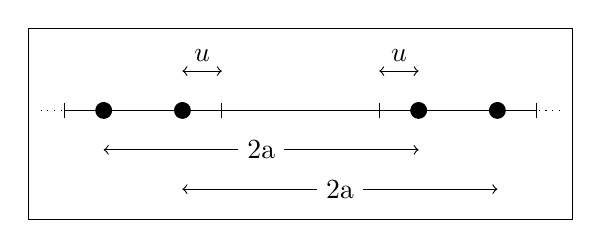
\begin{tikzpicture}[show background rectangle, scale = 1]
		\pgfmathsetmacro{\j}{0.5};
		\draw (0,0) -- (6,0);
		\foreach \i in {0,2,...,6}{
			\draw[fill = black] ({\i + \j * (-1)^(\i/2)},0) circle (0.1);
			\draw[] (\i,-0.1) -- (\i, 0.1);
		}
		\draw[<->] (2 - \j, -1) -- (6 - \j, -1) node[midway, fill = white] {2a};
		\draw[<->] (0 + \j, -0.5) -- (4 + \j, -0.5) node[midway, fill = white] {2a};
		\draw[<->] (2 - \j, 0.5) -- (2, 0.5) node[midway, above] {$u$};
		\draw[<->] (4, 0.5) -- (4 + \j, 0.5) node[midway, above] {$u$};
		\draw[dotted] (-0.3,0) -- (6.3, 0);
	\end{tikzpicture}
	\caption{Scheme: perfectly dimerized molecule}
	\label{image_scheme_dimer}
	\end{minipage}
\end{figure}
Assuming that the $\sigma$-binding energy can be expanded to second order about the symmetric state using an effective spring constant $\kappa$, the energy contribution can be written as:
\begin{align}
	\frac{\kappa}{2}\sum_n (u_{n+1} - u_n)^2
\end{align}
The $\pi$-binding energy is described in the earlier derived tight-binding approximation\footnote{Since the description is spinless, an additional factor of 2 is obtained.}. Finally the term of the kinetic energy of the atoms is added to get the so called \emph{SSH-Hamiltonian} (named after \textsc{W. P. Su, J. R. Schrieffer, A. J. Heeger}, see \cite{PhysRevB.22.2099, RevModPhys.60.781}):
\begin{align}
	\mathcal{H}_\text{SSH} &= \underbrace{-2\sum_{n} t_{n+1,n}\left(c_{n+1}^\dagger c_n + c_n^\dagger c_{n+1}\right)}_{\text{electron hopping / $\pi$-binding energy}} +
	\underbrace{\frac{1}{2}\sum_n \kappa (u_{n+1} - u_n)^2}_{\sigma-\text{binding energy}} + 
	\underbrace{\frac{1}{2} \sum_n M \dot{u}^2_n}_{\text{kinetic energy}}
\end{align}
Using \textsc{Born-Oppenheimer} approximation and a perfect symmetric dimerization $u_n = (-1)^nu$ (see \cref{image_scheme_dimer}) the Hamiltonian can be written as:
\begin{align}
	\mathcal{H} &= -2\sum_n \left[t_0 + (-1)^n\delta\right]\cdot\left(c_{n+1}^\dagger c_n + c_n^\dagger c_{n+1}\right) + 2N\kappa u^2\\
	&= -2\sum_n^{N_d} \left[\left(t_0+\delta\right)\left(c_{2n+1}^\dagger c_{2n} + c_{2n}^\dagger c_{2n+1} \right) + 
	\left(t_0-\delta\right)\left(c_{2n}^\dagger c_{2n-1} + c_{2n-1}^\dagger c_{2n} \right)\right]+2N\kappa u^2
\end{align}
Calculation of the $k$-space representations of the creation and annihilation operators finally leads to the expression:
\begin{align}
\mathcal{H} &= \sum_k \left[
\left(\epsilon_k + i\Delta_k\right)c_{k}^{\dagger(e)}c_{k}^{(o)} + \left(\epsilon_k-i\Delta_k \right)	c_{k}^{\dagger(o)}c_{k}^{(e)}\right] + 2N\kappa u^2
\end{align}
with the substitutions $\epsilon_k := 2t_0\cos(ka)$ and $\Delta_k := 2\delta\sin(ka)$. Here $c^{\dagger(e)}_k$, $c^{\dagger(o)}_k$, $c^{(e)}_k$, $c^{(o)}_k$ are the creation and annihilation operators at the even/odd $(e)$/$(o)$ positions to a certain $k$-point. Due to the displacement the primitive cell length doubled and therefore the first \textsc{Brillouine} zone goes only from $\nicefrac{-\pi}{2a}$ to $\nicefrac{\pi}{2a}$.\\
In further calculations the term $2N\kappa u^2$ will be neglected since it's only causing an offset. Thus the contribution of the Hamiltonian responsible for the form of the band structure is given by the terms:
\begin{align}
	\mathcal{H}_k &=
	\left[\epsilon_k + i\Delta_k\right]c_{k}^{\dagger(e)}c_{k}^{(o)} + \left[\epsilon_k-i\Delta_k \right]	c_{k}^{\dagger(o)}c_{k}^{(e)}
\end{align}
\begin{figure}
	\centering
	\begin{subfigure}{0.49\textwidth}
		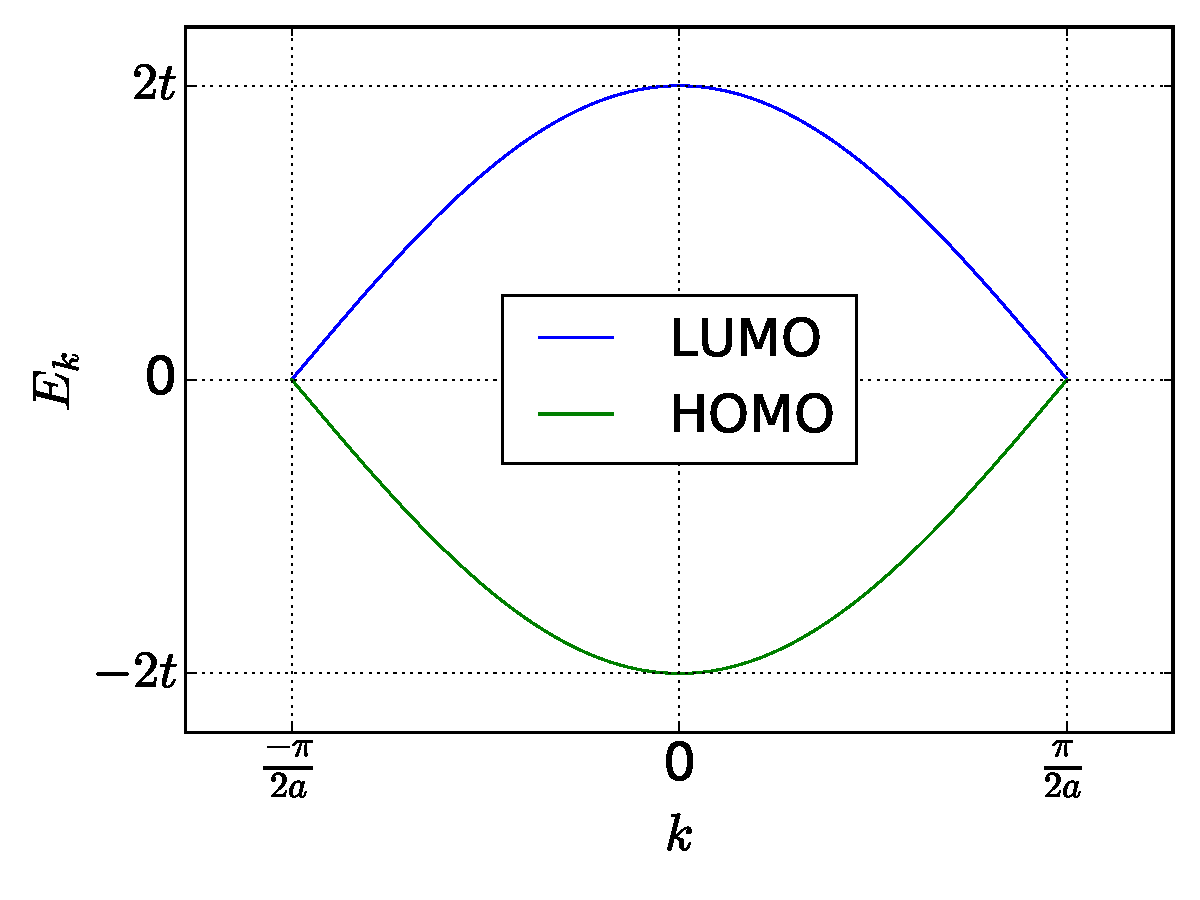
\includegraphics[width =\textwidth]{Images/Plots/bandstructure_without_gap}
		\caption{Band structure for no distortion ($u = 0$) leading to no band gap}
		\label{image_bs_wo_gap}
	\end{subfigure}\hspace*{0.2cm}
	\begin{subfigure}{0.49\textwidth}
		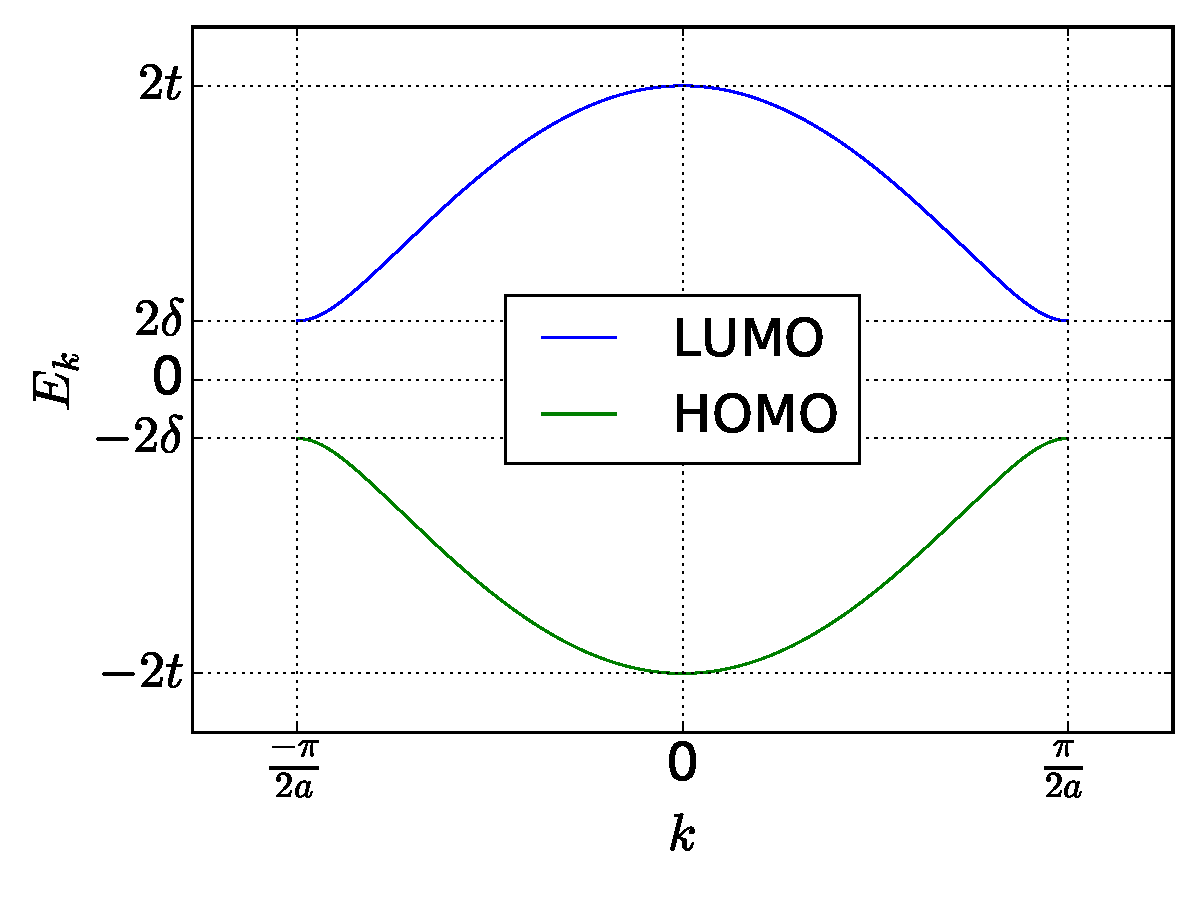
\includegraphics[width = \textwidth]{Images/Plots/bandstructure_with_gap}
		\caption{Band structure for distortion ($u \neq 0$) leading to a band gap of $4\delta$}
		\label{image_bs_w_gap}
	\end{subfigure}
	\caption{Structure of the HOMO- and LUMO-band arising from a tight-binding treatment of next-neighbor-hopping}
	\label{images_bs}
\end{figure}
with the eigenvalues\footnote{Note, that the $E_k$ are eigenvalues to single particle Hamiltonians} (see \cref{images_bs}):
\begin{align}
	E_k &= \pm \sqrt{\epsilon_k^2+\Delta_k^2}
	\label{equation_energy_band}
\end{align}
and the eigenstates:
\begin{align}
	\Psi_k^{(c)} &= \frac{1}{\sqrt{2}}\left(c_k^{\dagger(e)}+\frac{\epsilon_k - i \Delta_k}{|E_k|}c_{k}^{\dagger(o)}\right)
	\label{equation_conduction_eigenstate}\\
	\Psi_k^{(v)} &= \frac{1}{\sqrt{2}}\left(c_k^{\dagger(e)}-\frac{\epsilon_k - i \Delta_k}{|E_k|}c_{k}^{\dagger(o)}\right)
	\label{equation_valence_eigenstate}
\end{align}
corresponding to the valance $(v)$ and conduction $(c)$ band. Hereby the eigenfunctions have to be understood as operating on the vacuum state, $|(e),(o)\rangle = |0,0\rangle$. Thus the following relations can easily be shown:
\begin{align}
	\left\langle\Psi_k^{(\lambda)}\Big|\Psi_k^{(\lambda\prime)}\right\rangle &= \delta_{\lambda,\lambda\prime}\\
	\left\langle\Psi_k^{(v)}\Big|\mathcal{H}_{k}\Big|\Psi_k^{(v)}\right\rangle &= - |E_k|\\
	\left\langle\Psi_k^{(c)}\Big|\mathcal{H}_{k}\Big|\Psi_k^{(c)}\right\rangle &= |E_k|
\end{align}
It can also be shown, that the sum over the HOMO-band energies takes the form:
\begin{align}
E_0(u) &=-2\sum_k |E_k|\\
&=\frac{-4Nt_0}{\pi}\underbrace{\int\limits_{0}^{\nicefrac{\pi}{2}}\text{d}\theta\ \sqrt{1-\left(1-\frac{\delta^2}{t_0^2}\right)\sin^2(\theta)}}_{=:F(\nicefrac{\delta}{t_0})}
\end{align}
Here $F\left(\nicefrac{\delta}{t_0}\right)\approx 1$ for $\nicefrac{\delta}{t_0} \ll 1$.

\listoffigures
\listoftables
\bibliography{Chapters/literature}
\bibliographystyle{unsrtdin}
\label{here}
\end{document}



